%% thesis-p1.tex
%% Standalone P1 progress report entry point.
%% This file intentionally reuses the stable thesis chapter modules and does not modify thesis.tex.

\documentclass[english,singlespacedlisttitles]{umalayathesis}

\usepackage{lipsum}
\usepackage[utf8]{inputenc}
\usepackage[T1]{fontenc}
\usepackage{microtype}
\usepackage{graphicx}
\usepackage[dvipsnames,x11names,rgb]{xcolor}
\usepackage{tikz}
\usetikzlibrary{shapes.geometric, arrows, positioning, fit, calc}
\usepackage{pgfplots}
\pgfplotsset{compat=1.17}
\usepackage{url}
\usepackage{float}

\usepackage{listings}
\lstset{language=[LaTeX]TeX,columns=fullflexible,
        basicstyle=\ttfamily\SingleSpacing,
        texcsstyle=*\bfseries\color{NavyBlue},
        commentstyle=\itshape\color{PaleVioletRed4},
        frame=single,framesep=6pt,
        framexleftmargin=6pt,framexrightmargin=6pt,
        xleftmargin=12pt,xrightmargin=12pt,
        breaklines=true,breakatwhitespace=true,
}

\usepackage{longtable}
\usepackage{supertabular}
\usepackage{algorithm}
\usepackage{algorithmic}

\author{Tong Siyuan}
\title{Nano-Mamba U-Net: A Spatio-Temporal Framework for Cardiac Motion Analysis}
\othertitle{Nano-Mamba U-Net: Rangka Kerja Ruang-Masa untuk Analisis Pergerakan Jantung}
\university{Universiti Malaya}
\faculty{Faculty of Computer Science and Information Technology}
\submissionyear{2026}
\degree{Master of Artificial Intelligence}

\loadglsentries{myacronyms}

\begin{document}
\frontmatter

\makecoverandtitlepage{\mastercoursework}

{\clearpage
\tableofcontents\clearpage
\listoffigures\clearpage
\listoftables\clearpage
}

\mainmatter

% P1 required scope according to the MAI project briefing:
% Chapter 1: Introduction
% Chapter 2: Research Problem
% Chapter 3: Research Objectives
% Chapter 4: Literature Review
% Chapter 5: Research Design/Methodology
%!TEX ROOT = thesis.tex

% =========================================================
% CHAPTER 1: INTRODUCTION
% =========================================================
\chapter{INTRODUCTION}
\label{chap:intro}

\section{Background of the Study}

\subsection{Clinical Significance of Cardiovascular Diseases}
Cardiovascular diseases (CVDs) remain one of the most important global causes of mortality. According to the World Health Organization (WHO), CVDs caused an estimated 19.8 million deaths in 2022, corresponding to approximately 32\% of all global deaths \citep{who2025cvd}. This figure is not used in this thesis as a direct claim about the performance of any computational model. Rather, it establishes the clinical context in which efficient and reproducible cardiac image analysis tools are valuable. Given this burden, even a modest improvement has practical relevance if it makes cardiac assessment more dependable or easier to deliver at scale.

Cardiac Magnetic Resonance (CMR) imaging offers a non-invasive means of examining cardiac anatomy and function \citep{bernard2018deep}. It allows clinicians to obtain functional indices including Ejection Fraction (EF), End-Diastolic Volume (EDV), End-Systolic Volume (ESV), and Myocardial Mass. Reliable calculation of these indices requires separate masks of the myocardium (MYO) and the two ventricular cavities, LV and RV. Automated delineation consequently forms a core step in computer-assisted cardiac assessment. The experiments in this project first assess spatial segmentation at ED and ES. The selected Nano-Mamba checkpoint is subsequently run over every phase of each complete cine sequence to obtain phase timing, EF, ventricular volume trajectories, and global segmentation-derived motion surrogates.

The connection between a segmentation mask and a quantitative cardiac index can be illustrated with ventricular volume. If $V_{ED}$ is the ventricular volume at end-diastole and $V_{ES}$ is the volume at end-systole, ejection fraction is given by:
\begin{equation}
    EF = \frac{V_{ED}-V_{ES}}{V_{ED}}\times 100\%.
\end{equation}
The formula makes the consequence of a segmentation error explicit. A small boundary error can change the estimated cavity volume, and the resulting volume error can propagate into EF. In the completed full-cine analysis, the same relationship is evaluated at the manually labelled ED/ES endpoints and used to construct a complete segmentation-derived LV-volume trajectory.

\subsection{The Bottleneck of Manual Delineation and Traditional Methods}
Manual delineation of cardiac structures requires expert knowledge and substantial effort. A cine CMR study may contain many slices and cardiac phases. The ACDC challenge paper identifies both the diagnostic importance of accurately segmenting RV, MYO, and LV and the possibility of inter-observer variation in manual annotations \citep{bernard2018deep}. No single annotation-time estimate is assumed here because the available evidence does not support one. The relevant limitation is operational: a trained reader must contour each case, and the workload grows with the number of studies.

Manual contouring also involves judgement rather than simple tracing. Papillary muscles can obscure the boundary of the ring-shaped myocardium, and the RV has both a thin wall and marked geometric variation. Basal and apical slices introduce another ambiguity because cardiac structures appear or disappear gradually as the imaging plane changes. Two experts may therefore draw different contours on the same image. Automation does not replace that expertise; it provides a consistent initial result that a clinician can inspect before measurements are made.

Earlier segmentation pipelines used methods such as thresholding, active contours, level sets, and graph cuts. Their behaviour often depends on a chosen feature set, an initial contour, or a particular model of image intensity. CMR does not satisfy these conditions reliably: scanner-dependent contrast, partial-volume effects, papillary muscles, and indistinct boundaries all affect the image \citep{chen2020cardiacreview}. These limitations helped shift the field towards models whose representations are fitted from annotated data.

\subsection{Deep Learning for Cardiac Segmentation}
Deep learning changed this workflow by learning image features during training. Fully Convolutional Networks (FCNs) showed that a network could produce a dense semantic label map \citep{long2015fully}. U-Net then paired an encoder and decoder with skip connections, a design that became widely used in biomedical segmentation \citep{ronneberger2015u}; 3D U-Net extended it to volumetric convolutions \citep{cicek20163d}. The present work builds on these established architectures and does not claim them as new contributions.

A convolutional kernel sees only a local neighbourhood at each operation. For example, a $3\times3\times3$ kernel initially combines information from nearby voxels; a wider effective field emerges only after several layers are stacked. Cardiac MRI nevertheless requires both fine boundary evidence and knowledge of how the chambers and myocardium are arranged. The network must therefore separate myocardium from blood pool along local boundaries without losing the relative spatial organization of RV, MYO, and LV.

Transformer-based architectures address long-range interactions through self-attention \citep{vaswani2017attention,dosovitskiy2020image}. Medical segmentation models such as UNETR and Swin UNETR demonstrate the usefulness of global or window-based token interactions in volumetric segmentation tasks \citep{hatamizadeh2022unetr,hatamizadeh2022swin}. However, self-attention can increase memory and computational requirements, which motivates research into more efficient sequence modeling alternatives. This thesis does not argue that Transformers are unsuitable for medical imaging. Instead, it investigates whether a lighter sequence-inspired bottleneck can be useful when the hardware environment is constrained.

\subsection{Motivation for a Mamba-Inspired Bottleneck}
Selective State Space Models (SSMs), including Mamba, have recently attracted attention because they can model long sequences with linear-time complexity \citep{gu2023mamba}. This thesis investigates whether a lightweight Mamba-inspired sequence bottleneck can be integrated into a 3D U-Net-style architecture for cardiac MRI segmentation. The implemented model serializes compressed 3D volumetric features into a one-dimensional token sequence, applies a lightweight gated sequence module inspired by Mamba, and reshapes the result back into volumetric form.

The motivation is based on the accuracy-efficiency trade-off. A model with the highest Dice score is not necessarily the most suitable model for all environments if it requires more memory, more parameters, or longer inference time. Conversely, a very small model is not useful if it fails to segment clinically relevant structures. This thesis therefore evaluates Nano-Mamba U-Net not only by segmentation accuracy but also by parameter count and inference speed. The research question is whether a compact sequence-inspired bottleneck can produce competitive validation performance while maintaining a small model size.

The completed empirical design has two linked stages. In the historical six-model experiment, labelled ED and ES volumes are processed as independent 3D cases and tensor depth contains anatomical slices rather than time. In a separate post-hoc stage, the selected spatial Nano-Mamba checkpoint is applied to every frame of each validation cine. Fixed adjacent-frame probability fusion is then evaluated against frame-wise inference. From the resulting native-grid masks, the analysis derives ventricular volume trajectories together with ED/ES timing and EF. Motion is summarized separately through a global myocardial radial-distance surrogate and LV-centroid displacement. The project therefore completes a segmentation-derived spatio-temporal analysis, while stopping short of claiming a learned temporal Mamba network, optical flow, dense deformation, or regional strain.

\section{Scope of the Study}
The scope of this research is defined as follows:
\begin{itemize}
    \item \textbf{Dataset Boundary:} The empirical evaluation uses the Automated Cardiac Diagnosis Challenge (ACDC) dataset \citep{bernard2018deep}. The segmentation targets are RV, MYO, and LV.
    \item \textbf{Task Boundary:} The trained backbone performs four-class 3D cardiac MRI segmentation and treats ED/ES cases independently. A separate full-cine workflow evaluates frame-wise inference and fixed temporal probability fusion across 550 validation frames, then derives global volume, phase, EF, centroid-displacement, and myocardial-radius trajectories. Slice depth is never treated as time.
    \item \textbf{Implementation Boundary:} The proposed Nano-Mamba U-Net uses a Mamba-inspired bottleneck implemented in PyTorch. It should not be interpreted as a full reproduction of the original hardware-aware selective scan implementation.
    \item \textbf{Evaluation Boundary:} The main reported results are based on a deterministic patient-level 80/20 validation split of the ACDC training cohort. The study does not claim performance on the hidden official ACDC test set.
    \item \textbf{Hardware Boundary:} Training, validation, and computational profiling were conducted on a single consumer-grade NVIDIA RTX 4060 GPU with 8GB VRAM. Reported FPS is specific to the implemented batch-one benchmark and is not treated as a universal property of an architecture.
\end{itemize}
The scope statements above define how the results are to be read. This is a reproducible project-level investigation; it is neither a claim of clinical readiness nor evidence that the proposed model outperforms every cardiac segmentation method.

\section{Organization of the Thesis}
The thesis proceeds from context to evidence. Chapter 1 introduces the clinical and computational motivation, Chapter 2 defines the research problem, and Chapter 3 states the objectives and questions. The relevant convolutional, attention, residual, and state-space literature is reviewed in Chapter 4. Chapter 5 then records the data, preprocessing, model architecture, training, and evaluation protocol. Chapters 6 and 7 present and interpret the validation results, respectively, before Chapter 8 draws the conclusions and outlines future work.

% =========================================================
% CHAPTER 2: RESEARCH PROBLEM
% =========================================================
\chapter{RESEARCH PROBLEM}
\label{chap:problem}

An accurate segmentation score is necessary, but it is not the only design consideration for automated cardiac MRI. The model also has to run within available computing resources and handle the anatomical variation present across patients. This study therefore examines three connected difficulties in building a lightweight volumetric segmenter: limited contextual reach, computational cost, and variable cardiac anatomy.

\section{Local Context Modeling in Lightweight 3D CNNs}
3D CNNs process neighbouring voxels together, which is useful for volumetric segmentation. Their reach at one layer is nevertheless limited: a standard $3 \times 3 \times 3$ kernel only observes the surrounding voxels. Deeper stacks expand that reach, but depth and channel width are precisely what a small model must restrict. As a result, relationships across the heart may be represented incompletely, especially on basal and apical slices where the RV, MYO, and LV contours are uncertain. At such locations, similar local intensities can belong to different structures, so anatomical position and the surrounding chamber arrangement provide useful evidence beyond the immediate kernel.

Convolution remains the main operation in the proposed U-Net and is not being rejected. The practical issue is how much context survives when a small network compresses its features. Here, the bottleneck grid is written as a raster sequence and passed through a compact gated transformation. Mixing occurs over a kernel of three positions; the implemented block has neither selective state propagation nor direct all-token interaction. Its deliberately narrow role is why it supplements the compressed bottleneck instead of replacing the full U-Net with a large attention architecture. Operating after compression also keeps the sequence short enough for the available hardware. The experiment consequently evaluates a small addition to the convolutional backbone rather than a competing end-to-end sequence model.

\section{Computational Cost of Larger Segmentation Models}
Additional layers, channels, residual blocks, or attention operations can give a segmentation model more capacity. They also tend to increase its parameter count and may raise memory use or inference cost. Where hardware is limited, a small loss in Dice can be acceptable if it buys a substantial reduction in model size. The comparison in this thesis is therefore concerned with the observed accuracy--efficiency balance, not with Dice in isolation. Neither side of that balance is assumed in advance: segmentation quality and resource indicators are reported together for the executed models.

For that reason, the evaluation places parameter count and measured inference speed beside Dice. The term \emph{lightweight} is used here in a specific sense: the model has the lowest reported trainable-parameter count and competitive batch-one throughput on the recorded hardware. It is not claimed to lead simultaneously in memory, speed, and accuracy. Thus, the 1.46M-parameter Nano model can still be useful when a larger model attains a higher Dice, provided that the saving is material. All baselines and ablations are compared under the same data split and training protocol so that this trade-off can be examined consistently.

\section{Pathological and Anatomical Variability}
Besides normal cases, ACDC contains myocardial infarction, hypertrophic cardiomyopathy, dilated cardiomyopathy, and right-ventricular abnormality \citep{bernard2018deep}. These diagnoses introduce differences in chamber size, myocardial thickness, and boundary appearance. The validation data therefore include both normal hearts and anatomy altered by disease.

Anatomical variation is especially troublesome for the RV and MYO masks. The RV is thin-walled and irregular, while the myocardium occupies a narrow ring. A displacement of only a few voxels can therefore affect their overlap scores more strongly than it would affect a larger cavity. Reporting RV, MYO, and LV separately makes this behaviour visible instead of hiding it inside one mean Dice value. It also shows whether a change in the overall average reflects broad improvement or is driven mainly by the easier ventricular cavity.

\section{From Endpoint Segmentation to Cardiac-Cycle Analysis}
Manual labels at ED and ES make endpoint segmentation evaluation possible, but they do not show what the model predicts between those phases. Applying the spatial checkpoint to every cine frame fills that gap with a sequence of masks. Because the frames were not trained jointly, however, adjacent predictions can fluctuate. Examining the complete curve makes those jumps visible and permits phase and functional measurements that cannot be obtained from one isolated endpoint mask. The research problem is thus to connect the validated spatial checkpoint to a transparent time-series analysis while keeping it distinct from a learned four-dimensional network. The approach used here applies fixed circular probability fusion and assesses endpoint overlap, EF, phase timing, curve smoothness, and global motion surrogates. Manual endpoint labels provide partial validation, while the absence of intermediate-frame labels remains a stated limitation.

\section{Research Gap}
Existing segmentation backbones such as 3D U-Net, Attention U-Net, and SegResNet provide strong baselines, but they represent different points on the accuracy-efficiency spectrum. The first research gap addressed in this thesis is whether a compact Mamba-inspired bottleneck can provide competitive validation performance with fewer parameters than conventional or residual alternatives, while remaining feasible on a consumer GPU. The second is whether the selected spatial checkpoint can support a reproducible full-cine, segmentation-derived function and global motion analysis, and whether a fixed temporal fusion produces a measurable change relative to independent frame-wise inference.

The gap is not a claim that previous methods are inadequate in all settings. SegResNet, for example, remains a strong residual convolutional baseline. The gap is narrower and more appropriate for this project: there is value in testing a compact sequence-inspired bottleneck under a rigorous patient-level validation protocol, especially when earlier exploratory scripts may overestimate performance by evaluating on non-held-out data. This thesis therefore emphasizes reproducibility and honest comparison as much as architectural novelty.

% =========================================================
% CHAPTER 3: RESEARCH OBJECTIVES
% =========================================================
\chapter{RESEARCH OBJECTIVES}
\label{chap:objectives}

The aim of this research is to design, implement, and evaluate a lightweight Mamba-inspired U-Net architecture for cardiac MRI segmentation and to determine how its segmentations can support a bounded full-cine cardiac motion and function analysis. Empirical validation is central to the study: parameter efficiency is assessed alongside established baselines, and spatial learning is kept conceptually separate from the post-hoc temporal stage. The objectives connect directly to the experiments reported in Chapter 6.

\section{Specific Objectives}
\begin{enumerate}
    \item To implement a Nano-Mamba U-Net architecture that inserts a lightweight Mamba-inspired sequence bottleneck into a 3D U-Net-style encoder-decoder network.
    \item To evaluate the segmentation performance of the proposed model on RV, MYO, and LV using Dice Similarity Coefficient on a deterministic patient-level validation split of the ACDC training cohort.
    \item To compare the proposed model with 3D U-Net, Attention U-Net, SegResNet, and ablation variants using the same split, preprocessing, epoch budget, optimizer family, and validation protocol, with model-specific batch sizes disclosed as a limitation.
    \item To quantify computational efficiency using reported trainable-parameter count and batch-one inference speed.
    \item To apply the selected Nano-Mamba checkpoint to complete validation cine sequences, derive segmentation-based cardiac volume, phase, EF, and global motion trajectories, and quantify what fixed adjacent-frame probability fusion changes relative to independent frame-wise inference.
\end{enumerate}

The first objective is implemented through the model architecture described in Chapter 5. The second and third objectives are addressed through the six-model quantitative validation table in Chapter 6. The fourth objective is addressed by reporting trainable parameters and inference speed together with Dice. The fifth objective is addressed by the independently audited 20-patient, 550-frame full-cine analysis. This mapping ensures that every stated objective is answered by an implemented experiment.

\section{Research Questions}
\begin{enumerate}
    \item How can compressed 3D cardiac MRI feature maps be serialized and processed by a Mamba-inspired bottleneck within a U-Net-style segmentation architecture?
    \item Does the proposed Nano-Mamba U-Net achieve competitive held-out validation Dice compared with 3D U-Net, Attention U-Net, SegResNet, and ablation variants?
    \item What accuracy-efficiency trade-off is observed when comparing Nano-Mamba U-Net with heavier or non-Mamba alternatives in terms of Dice score, parameter count, and inference speed?
    \item How can the selected spatial segmentation checkpoint support full-cine cardiac function and global motion analysis, and what measurable effect does fixed adjacent-frame probability fusion have relative to frame-wise inference?
\end{enumerate}

These research questions are intentionally phrased in a measurable way. The first question is answered by architecture implementation rather than by a numerical score alone. The second question is answered by held-out validation Dice. The third question is answered by jointly interpreting Dice, parameter count, and speed. The fourth is answered by complete cine coverage, endpoint validation, functional and motion-derived quantities, and paired temporal-fusion comparisons. Each answer must therefore follow from an implemented analysis; neither absolute superiority nor dense motion tracking can be inferred from these questions.

%!TEX ROOT = thesis.tex

% =========================================================
% CHAPTER 4: LITERATURE REVIEW
% =========================================================
\chapter{LITERATURE REVIEW}
\label{chap:litreview}

This chapter reviews the scientific and technical literature that supports the design choices of this thesis. The purpose is not to claim that the proposed model replaces all existing cardiac segmentation methods. Instead, the review identifies the specific research context in which a lightweight Mamba-inspired U-Net is meaningful: automated cardiac MRI segmentation requires accurate anatomical delineation, but practical models must also consider parameter count, memory usage, and reproducible validation.

\section{Cardiac MRI Segmentation as a Clinical Computing Problem}
Cardiac Magnetic Resonance (CMR) imaging is widely used for non-invasive assessment of cardiac morphology and function. In the ACDC benchmark, the segmentation targets are the Right Ventricle (RV), Myocardium (MYO), and Left Ventricle (LV), which are clinically important because they support the computation of ventricular volumes, myocardial mass, and ejection fraction \citep{bernard2018deep}. These quantities are not obtained directly from a neural network classifier; they require spatial masks from which anatomical volumes can be computed. Therefore, segmentation quality is central to the reliability of downstream cardiac function analysis.

CMR segmentation is challenging because the difficulty is not uniform across all structures. LV segmentation is often more stable because the LV cavity is relatively compact and has a clearer blood-pool boundary. In contrast, the myocardium is a thin ring-like structure whose boundaries can be affected by partial volume effects, papillary muscles, and signal ambiguity. The RV is also difficult because it has a more variable crescent-like shape and thinner wall. These anatomical observations explain why a single aggregate Dice score is insufficient; class-specific performance should also be reported when evaluating cardiac segmentation models.

The ACDC dataset is useful for this thesis because it includes multiple cardiac conditions, including normal subjects and pathological groups such as dilated cardiomyopathy, hypertrophic cardiomyopathy, myocardial infarction, and abnormal right ventricle cases \citep{bernard2018deep}. This heterogeneity makes the benchmark more relevant than a dataset containing only healthy cardiac anatomy. Nevertheless, the ACDC training cohort remains a limited dataset, so patient-level separation between training and validation is essential. If frames from the same patient appear in both training and evaluation, the reported performance may reflect memorization of patient-specific anatomy rather than generalization.

\section{Traditional Medical Image Segmentation Methods}
Before deep learning became dominant, medical image segmentation commonly relied on intensity thresholding, deformable models, graph-based optimization, and level-set methods. These approaches remain important historically because they clarify why learning-based segmentation became attractive.

A simple thresholding method assumes that the target object can be separated from the background by intensity. Otsu's method, for example, selects a threshold $T$ by maximizing the between-class variance \citep{otsu1979threshold}. If the two classes have probabilities $\omega_0(T)$ and $\omega_1(T)$, and means $\mu_0(T)$ and $\mu_1(T)$, the objective can be written as:
\begin{equation}
    \sigma_B^2(T) = \omega_0(T)\omega_1(T)\left[\mu_0(T)-\mu_1(T)\right]^2.
\end{equation}
This formulation is elegant because it does not require annotated training data. However, it is not sufficient for cardiac MRI segmentation. MRI intensities are not standardized in the same way as CT Hounsfield Units, and myocardium, blood pool, and surrounding tissues may overlap in intensity. As a result, a global threshold cannot reliably separate RV, MYO, and LV across patients.

Active contour models, introduced by \citet{kass1988snakes}, formulate segmentation as an energy minimization problem. A contour evolves under internal smoothness forces and external image forces. A simplified energy functional can be written as:
\begin{equation}
    E_{snake} = \int_0^1 \left[\frac{1}{2}\alpha |v'(s)|^2 + \frac{1}{2}\beta |v''(s)|^2 + E_{image}(v(s))\right]ds.
\end{equation}
Here, the first two terms regulate contour continuity and smoothness, while $E_{image}$ attracts the contour to image features such as edges. This is useful when boundaries are clear, but cardiac MRI boundaries can be weak or ambiguous at basal and apical slices. Moreover, deformable models often require careful initialization, which limits their practicality for fully automated pipelines.

Level-set methods represent the contour implicitly as the zero level of a higher-dimensional function $\phi$ \citep{osher1988fronts}. A typical evolution equation is:
\begin{equation}
    \frac{\partial \phi}{\partial t} + F|\nabla \phi| = 0.
\end{equation}
The implicit representation allows topology changes more naturally than parametric snakes. However, iterative numerical optimization and sensitivity to image forces remain practical limitations. For this reason, traditional methods are useful background, but they do not remove the need for robust data-driven segmentation in heterogeneous CMR datasets \citep{chen2020cardiacreview}.

\section{Deep Learning Segmentation Architectures}
\subsection{Fully Convolutional Networks and U-Net}
Fully Convolutional Networks (FCNs) showed that classification-style neural networks could be reformulated for dense pixel-wise prediction by replacing fully connected layers with convolutional operations \citep{long2015fully}. This idea was important because segmentation requires a prediction for every pixel or voxel rather than one image-level label.

U-Net became one of the most influential architectures in biomedical image segmentation \citep{ronneberger2015u}. Its main contribution is the encoder-decoder structure with skip connections. The encoder gradually reduces spatial resolution to learn semantic features, while the decoder restores resolution to produce a segmentation mask. Skip connections transfer high-resolution spatial features from the encoder to the decoder, which helps recover fine boundaries. If $\mathbf{X}^{(l)}_{enc}$ is an encoder feature map and $\mathbf{X}^{(l+1)}_{dec}$ is a decoder feature map from a coarser level, a simplified skip-connection operation can be written as:
\begin{equation}
    \mathbf{X}^{(l)}_{\mathrm{dec}}
    =\operatorname{Conv}\!\left(
      \operatorname{Concat}\!\left[
        \mathbf{X}^{(l)}_{\mathrm{enc}},
        \operatorname{Upsample}\!\left(\mathbf{X}^{(l+1)}_{\mathrm{dec}}\right)
      \right]
    \right),
\end{equation}
where \(\operatorname{Upsample}\) restores spatial resolution,
\(\operatorname{Concat}\) joins feature channels, and
\(\operatorname{Conv}\) performs convolutional refinement. Writing the
operations by name avoids any ambiguity about the order: up-sampling occurs
before channel concatenation, and convolution follows the concatenation. This
equation explains why U-Net is suitable for medical segmentation: the decoder
does not reconstruct boundaries only from compressed semantic features; it
also receives high-resolution information from earlier encoder layers.

For volumetric data, 3D U-Net extends the same principle from 2D images to 3D tensors \citep{cicek20163d}. V-Net also used volumetric convolution and Dice-based optimization for 3D medical segmentation \citep{milletari2016v}. These works are directly relevant to this thesis because the proposed Nano-Mamba U-Net uses a 3D U-Net-style encoder-decoder as its architectural base. The contribution of this thesis is not the invention of the U-Net framework itself. Rather, the project studies whether the bottleneck of such a framework can be modified into a compact sequence-processing module.

\begin{figure}[hbt!]
\centering
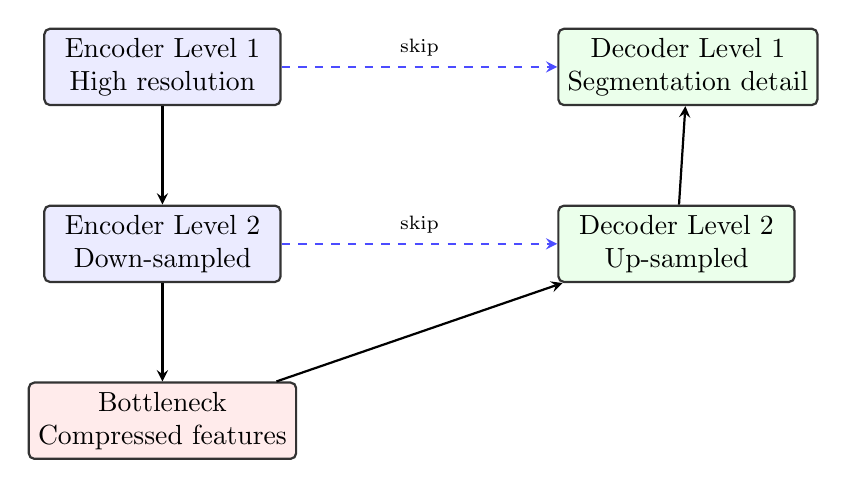
\begin{tikzpicture}[
    node distance=1.25cm and 1.4cm,
    block/.style={rectangle, draw=black!80, thick, rounded corners=2pt, minimum width=3.0cm, minimum height=0.85cm, align=center},
    enc/.style={block, fill=blue!8},
    dec/.style={block, fill=green!8},
    bot/.style={block, fill=red!8},
    arrow/.style={->, >=stealth, thick},
    skip/.style={->, >=stealth, dashed, thick, draw=blue!70}
]
\node[enc] (e1) {Encoder Level 1\\High resolution};
\node[enc, below=of e1] (e2) {Encoder Level 2\\Down-sampled};
\node[bot, below=of e2] (b) {Bottleneck\\Compressed features};
\node[dec, right=3.5cm of e2] (d2) {Decoder Level 2\\Up-sampled};
\node[dec, right=3.5cm of e1] (d1) {Decoder Level 1\\Segmentation detail};
\draw[arrow] (e1) -- (e2);
\draw[arrow] (e2) -- (b);
\draw[arrow] (b) -- (d2);
\draw[arrow] (d2) -- (d1);
\draw[skip] (e2) -- node[above, font=\scriptsize] {skip} (d2);
\draw[skip] (e1) -- node[above, font=\scriptsize] {skip} (d1);
\end{tikzpicture}
\caption{Conceptual encoder-decoder structure of U-Net-style segmentation models. Encoder blocks learn increasingly abstract features, decoder blocks recover spatial resolution, and skip connections preserve boundary information.}
\label{fig:unet_concept}
\end{figure}

\subsection{Attention U-Net}
Attention U-Net introduced attention gates to suppress irrelevant encoder features before they are passed through skip connections \citep{oktay2018attention}. This is relevant in medical images because large regions of an image may contain background structures unrelated to the target anatomy. In a simplified attention gate, an encoder feature $x$ and a decoder gating signal $g$ are projected into a shared representation and transformed into an attention coefficient:
\begin{equation}
    \alpha = \operatorname{sigmoid}\!\left(
      \boldsymbol{\psi}^{\mathsf{T}}
      \delta\!\left(W_xx + W_gg + b\right)
    \right).
\end{equation}
The filtered feature can then be represented as:
\begin{equation}
    \hat{x}_i=\alpha_i x_i,
\end{equation}
where index \(i\) runs over the spatial feature elements. Thus,
\(\operatorname{sigmoid}\) maps the attention score to a coefficient,
\(\delta\) is a nonlinear activation, and \(\alpha_i x_i\) is explicit
element-wise multiplication. The key idea is not that attention automatically
guarantees better segmentation, but that it provides a mechanism for feature
selection. In the final experiment of this thesis, Attention U-Net did not
outperform the other models, which illustrates why empirical comparison under
the same split is necessary.

\subsection{Residual Networks and SegResNet}
Residual learning was introduced to make deeper networks easier to optimize \citep{he2016deep}. Instead of asking stacked layers to learn a full mapping $H(x)$, a residual block learns a residual function $F(x)$ and adds the input back to the output:
\begin{equation}
    y = F(x) + x.
\end{equation}
This identity shortcut improves gradient flow and can make deeper convolutional models more trainable. SegResNet-style medical segmentation architectures use residual blocks in an encoder-decoder setting \citep{myronenko2019segresnet}. In this thesis, the MONAI SegResNet configuration with 16 initial filters serves as a residual convolutional alternative to the proposed Nano-Mamba U-Net. The final results show that SegResNet16 achieved the highest mean Dice, which must be acknowledged rather than hidden.

\section{Transformers and Sequence Modeling in Medical Imaging}
Transformers introduced self-attention as a way to model long-range dependencies \citep{vaswani2017attention}. Vision Transformer adapted this idea to image classification by treating image patches as tokens \citep{dosovitskiy2020image}. In medical imaging, UNETR used transformer encoders for 3D segmentation \citep{hatamizadeh2022unetr}, while Swin Transformer and Swin UNETR introduced hierarchical shifted-window attention to reduce the cost of global attention \citep{liu2021swin,hatamizadeh2022swin}.

The computational concern with standard self-attention is that the attention matrix grows quadratically with the number of tokens. For an input sequence of length $N$, the attention matrix has size $N\times N$, and the simplified attention operation is:
\begin{equation}
    \operatorname{Attention}(Q,K,V)
    =\left[
      \operatorname{softmax}\!\left(
        \frac{QK^{\mathsf{T}}}{\sqrt{d_k}}
      \right)
    \right]V.
\end{equation}
Here, \(d_k\) is the key-vector dimension. The square brackets make the
scope explicit: softmax acts on the complete scaled score matrix
\(QK^{\mathsf{T}}/\sqrt{d_k}\), and the resulting attention-weight matrix is
then multiplied by \(V\). This equation shows why sequence length matters: the
multiplication \(QK^{\mathsf{T}}\) compares every token with every other token.
Window-based methods reduce this cost, but the broader issue remains important
for volumetric segmentation because 3D images can produce many spatial tokens.

It would be inaccurate to claim that all transformer models are infeasible or that they are unsuitable for medical imaging. Prior work shows that transformer-based segmentation can be effective. The more careful motivation for this thesis is narrower: for a master's project focused on lightweight deployment and reproducible experiments on a consumer GPU, it is reasonable to investigate alternatives that attempt to combine broader context modeling with lower parameter count.

\section{State Space Models and Mamba-Inspired Design}
State Space Models (SSMs) represent sequence dynamics through a hidden state. A continuous-time linear state space model can be written as:
\begin{equation}
    h'(t)=Ah(t)+Bx(t), \qquad y(t)=Ch(t).
\end{equation}
Here, $h(t)$ is the hidden state, $x(t)$ is the input signal, $y(t)$ is the output signal, and $A$, $B$, and $C$ are state transition and projection matrices. In the context of deep learning, the appeal of SSMs is that they can model long sequences without explicitly constructing a full $N\times N$ attention matrix.

Mamba extends this line of work through selective state space modeling and hardware-aware sequence processing \citep{gu2023mamba}. Recent biomedical segmentation studies have also explored Mamba-style modules for medical image segmentation. U-Mamba combines convolutional processing with state-space blocks, while SegMamba studies long-range sequential modeling for 3D medical segmentation \citep{ma2024umamba,xing2024segmamba}. VM-UNet uses Visual State Space blocks in a U-shaped architecture, Mamba-UNet uses a VMamba-based encoder-decoder and reports experiments on ACDC and Synapse, and LightM-UNet uses residual Vision Mamba layers to pursue a lightweight design \citep{ruan2024vmunet,wang2024mambaunet,liao2024lightmunet}. These works make Mamba/SSM segmentation directly relevant to this thesis, but they are related methods rather than evidence that every Mamba-inspired block will automatically improve cardiac segmentation.

However, this thesis must distinguish the original Mamba implementation, the Visual State Space or SSM blocks in those recent segmentation models, and the implemented project model. Nano-Mamba serializes compressed 3D features and applies only kernel-3 depthwise sequence convolution, token-wise scalar gating, projections, and a residual connection. It has no recurrent state-space transition, selective scan, attention matrix, or direct global all-token interaction. Its fixed raster order also creates boundary adjacencies that are not isotropic 3D neighbours. It is therefore more accurate to describe the contribution as a local Mamba-inspired gated bottleneck exploration, not as a reproduction of Mamba or the cited Visual State Space architectures.

This distinction matters for scientific integrity. If the implementation does not include the full selective scan algorithm, the thesis should not claim that it has implemented the complete Mamba architecture. The contribution is still valid, but it should be framed correctly: the project investigates whether a compact sequence-inspired bottleneck can provide a useful accuracy-efficiency trade-off in cardiac MRI segmentation.

\section{Full-Cine Temporal Segmentation and Cardiac Motion Analysis}
Cardiac cine analysis can use time in fundamentally different ways. \citet{qin2018jointmotion} jointly learned cardiac MR segmentation and motion estimation using recurrent spatial transformers, thereby producing explicit inter-frame motion information in addition to masks. \citet{yan2019cineflow} used optical-flow learning to add the temporal dimension to cine MRI analysis. Such approaches seek a deformation field or pixel/tissue correspondence between phases; when appropriately validated, this supports motion tracking beyond independent mask measurements.

The present thesis addresses a narrower downstream problem. The trained Nano-Mamba backbone receives one 3D phase at a time and has no temporal input. After all phases are inferred, a fixed circular filter combines class probabilities as $0.25P_{t-1}+0.50P_t+0.25P_{t+1}$, including wrap-around at the first and last phases. The resulting masks support LV/RV/MYO volume curves, phase timing, EF, LV-centroid displacement, and a myocardial radial-distance summary. These are segmentation-derived global temporal and motion surrogates. They do not establish point correspondence, a dense deformation field, optical flow, local myocardial displacement, or strain. This distinction defines both the contribution and the validation boundary of the full-cine stage.

\section{Loss Functions and Evaluation Metrics}
Medical segmentation is often class-imbalanced because background voxels dominate the image volume, while structures such as myocardium occupy a smaller region. Dice-based objectives are commonly used because they directly optimize overlap between prediction and ground truth \citep{milletari2016v,sudre2017generalised}. For a predicted binary mask $P$ and ground-truth mask $G$, the Dice Similarity Coefficient is:
\begin{equation}
    \mathrm{DSC}(P,G)=\frac{2|P\cap G|}{|P|+|G|}.
\end{equation}
In multi-class segmentation, Dice can be computed separately for RV, MYO, and LV, and then averaged. This is the reporting strategy used in this thesis.

Cross-entropy is also widely used because it provides voxel-wise classification supervision. If $y_i$ is the true class at voxel $i$ and $p_{i,c}$ is the predicted probability for class $c$, the multi-class cross-entropy can be expressed as:
\begin{equation}
    L_{\mathrm{CE}}=-\sum_i\sum_c \mathbf{1}(y_i=c)\log p_{i,c}.
\end{equation}
The final experiment uses MONAI's Dice-Cross Entropy loss, combining region-overlap supervision with voxel-wise classification supervision. This choice is practical rather than novel; it follows established segmentation practice and is supported by the MONAI framework \citep{cardoso2022monai}.

Evaluation should also avoid leakage. If the same patient contributes samples to both training and validation, the measured Dice may overestimate generalization. Therefore, the final experimental design of this thesis uses patient-level splitting. This methodological point is as important as the architecture itself, because a strong model comparison is only meaningful when all models are trained and evaluated under the same split.

\section{Summary of the Literature Gap}
The literature shows that U-Net-style models remain strong foundations for biomedical segmentation, attention mechanisms can improve feature selection, residual models provide strong convolutional baselines, and transformer/SSM approaches offer explicit mechanisms for longer-range modeling. Recent Mamba segmentation studies include full Visual State Space or state-space components, whereas the present block is a substantially simpler local gated operation. The first gap addressed here is therefore not the absence of segmentation models, but the need to evaluate this compact implementation honestly under a reproducible patient-level protocol.

The motion literature also distinguishes segmentation-derived trajectories from learned motion fields and optical flow. The second gap addressed here is a bounded, auditable bridge from one validated spatial checkpoint to complete-cine global function and motion summaries, together with a direct comparison of frame-wise inference and fixed circular probability fusion. Based on this review, Nano-Mamba U-Net is positioned as a lightweight Mamba-inspired extension of a 3D U-Net-style model embedded in a complete but non-dense temporal analysis. The appropriate questions are whether it offers a useful accuracy--efficiency trade-off on ACDC and what its segmentation outputs can support without claiming learned temporal representation or tissue tracking.

%!TEX ROOT = thesis.tex

% =========================================================
% CHAPTER 5: RESEARCH DESIGN AND METHODOLOGY
% =========================================================
\chapter{RESEARCH DESIGN AND METHODOLOGY}
\label{chap:methodology}

This chapter establishes the rigorous methodological framework governing the development, optimization, and evaluation of the proposed Nano-Mamba U-Net. Moving beyond empirical heuristics, this section structurally justifies every engineering decision—from addressing the inherent physical artifacts of Magnetic Resonance Imaging (MRI) during preprocessing to formulating a mathematically robust optimization objective capable of mitigating severe anatomical class imbalances. Furthermore, this chapter provides an exhaustive architectural and mathematical deconstruction of the deep learning system itself, explicitly fulfilling the "Research Design" mandate by detailing the continuous-to-discrete state space transformations that empower the model.

\section{Dataset Justification and Clinical Heterogeneity}
The empirical validation of any deep learning architecture in medical imaging is profoundly dependent on the quality, diversity, and clinical realism of the utilized dataset. Deep neural networks are notoriously prone to overfitting to the specific scanner characteristics or healthy anatomical priors of a limited cohort \cite{campello2021multi}. To ensure the proposed model's robustness and clinical translatability, this research exclusively leverages the Automated Cardiac Diagnosis Challenge (ACDC) dataset \cite{bernard2018deep}.

The ACDC cohort consists of 100 distinct patients whose Cardiac Magnetic Resonance (CMR) cine sequences were acquired using 1.5T and 3.0T Siemens scanners. The defining characteristic of this dataset is its deliberate inclusion of severe pathological heterogeneity. The dataset is equally partitioned into five clinically distinct groups: Normal subjects (NOR), patients with previous Myocardial Infarction (MINF), Dilated Cardiomyopathy (DCM), Hypertrophic Cardiomyopathy (HCM), and Abnormal Right Ventricle (ARV). From an algorithmic perspective, these pathologies introduce extreme intra-class variability. For instance, in HCM patients, the myocardial wall is pathologically thickened, often blurring the boundaries with the papillary muscles, whereas in MINF patients, the presence of scar tissue severely alters the native magnetic resonance signal intensities and local image textures. The fundamental objective is to train the Nano-Mamba U-Net to learn highly abstract, pathology-invariant spatial representations to accurately segment the Right Ventricle (RV), Myocardium (MYO), and Left Ventricle (LV) across these diverse physical deformations.

\section{Data Harmonization and Spatial Resampling}
Medical imaging data generated in real-world clinical environments is inherently unstandardized. Variability in patient positioning, scanner FOV (Field of View), and institutional acquisition protocols lead to severe inconsistencies in physical voxel spacing and tensor dimensions. As demonstrated by the seminal work on the nnU-Net architecture \cite{isensee2021nnu}, the systematic harmonization of spatial metadata is arguably as critical to segmentation accuracy as the neural network architecture itself. 

The sequential progression of the data tensors through the preprocessing pipeline is structurally represented in Figure \ref{fig:preprocessing_pipeline}. This automated harmonization was rigorously implemented utilizing the MONAI (Medical Open Network for AI) framework \cite{cardoso2022monai}.

\begin{figure}[hbt!]
\centering
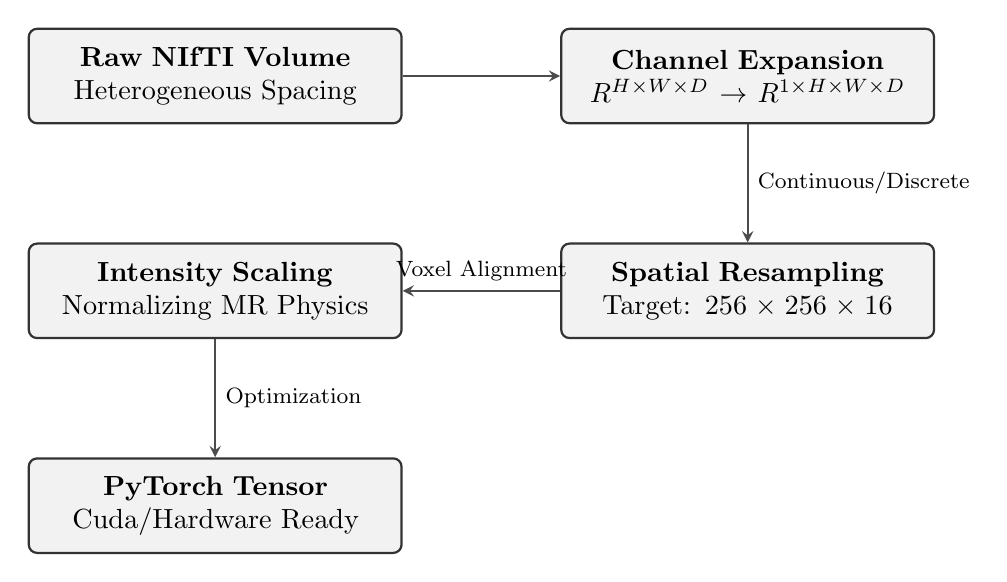
\begin{tikzpicture}[
    node distance=1.5cm and 2cm,
    block/.style={rectangle, draw=black!80, thick, fill=gray!10, text width=4.5cm, align=center, rounded corners=3pt, minimum height=1.2cm},
    arrow/.style={->, >=stealth, thick, draw=black!70}
]
% Nodes
\node[block] (raw) {\textbf{Raw NIfTI Volume}\\ Heterogeneous Spacing};
\node[block, right=of raw] (channel) {\textbf{Channel Expansion}\\ $\mathbb{R}^{H \times W \times D} \rightarrow \mathbb{R}^{1 \times H \times W \times D}$};
\node[block, below=of channel] (resample) {\textbf{Spatial Resampling}\\ Target: $256 \times 256 \times 16$};
\node[block, left=of resample] (intensity) {\textbf{Intensity Scaling}\\ Normalizing MR Physics};
\node[block, below=of intensity] (tensor) {\textbf{PyTorch Tensor}\\ Cuda/Hardware Ready};
% Arrows
\draw[arrow] (raw) -- (channel);
\draw[arrow] (channel) -- node[right, font=\footnotesize] {Continuous/Discrete} (resample);
\draw[arrow] (resample) -- node[above, font=\footnotesize] {Voxel Alignment} (intensity);
\draw[arrow] (intensity) -- node[right, font=\footnotesize] {Optimization} (tensor);
\end{tikzpicture}
\caption{The chronological data harmonization pipeline. Raw 3D MRI volumes undergo structural standardization to resolve spatial anisotropy and signal variability prior to network ingestion.}
\label{fig:preprocessing_pipeline}
\end{figure}

\subsection{Mathematical Formulation of Trilinear Interpolation}
To ensure structural compatibility with the Nano-Mamba tensor dimensions, all variable-sized volumes were spatially resampled to a standardized discrete grid of $256 \times 256 \times 16$. Because image intensities represent a continuous physiological signal captured at discrete spatial coordinates, mapping them to a new grid requires robust mathematical interpolation to prevent severe aliasing artifacts. 

For the continuous MRI intensity volumes, Trilinear Interpolation was applied. Let $V(x, y, z)$ denote the interpolated voxel intensity at a continuous Cartesian coordinate. By identifying the eight bounding discrete neighboring voxels $V_{000}$ through $V_{111}$ within the original grid, the continuous trilinear approximation is formulated as:
\begin{equation}
    V(x,y,z) \approx \sum_{i=0}^{1} \sum_{j=0}^{1} \sum_{k=0}^{1} V_{ijk} \cdot (1 - |x - x_i|) \cdot (1 - |y - y_j|) \cdot (1 - |z - z_k|),
\end{equation}
where $x_i, y_j, z_k$ represent the normalized spatial coordinates of the respective neighbors. 

Conversely, the ground-truth segmentation masks consist of strictly categorical integers (e.g., $1$ for RV, $2$ for MYO). Applying continuous polynomial interpolation to these masks would yield meaningless floating-point values, thereby destroying the categorical class definitions. Consequently, the label matrices are resampled utilizing Nearest-Neighbor Interpolation. This non-linear operation assigns the class of the closest original voxel by minimizing the Euclidean distance:
\begin{equation}
    V_{mask}(x, y, z) = V \left( \arg\min_{(x_i, y_i, z_i)} \sqrt{(x-x_i)^2 + (y-y_i)^2 + (z-z_i)^2} \right).
\end{equation}

\subsection{Addressing MR Intensity Heterogeneity}
Unlike Computed Tomography (CT), which relies on a standardized physical radiodensity scale (Hounsfield Units), the intensity values in MRI are relative and highly dependent on the specific acquisition parameters (e.g., echo time, repetition time) and the intrinsic magnetic field strength \cite{nyul1999on}. Consequently, the exact same myocardial tissue can manifest with drastically different numerical pixel intensities across different patients, creating severe instability during gradient descent optimization.

To construct a normalized feature space for the neural network, the spatial intensities are systematically bounded. The Min-Max scaling function $S(\mathcal{I})$ projects the continuous intensity range into a normalized subset $[0, 1]$:
\begin{equation}
    S(\mathcal{I}_{xyz}) = \frac{\mathcal{I}_{xyz} - \min(\mathcal{I})}{\max(\mathcal{I}) - \min(\mathcal{I}) + \epsilon},
\end{equation}
where $\epsilon = 10^{-8}$ serves as a negligible numerical stability constant designed to rigorously prevent division-by-zero singularities in the event of homogeneously black image slices.

\section{System Architecture Design: The Nano-Mamba U-Net}
The core "Research Design" of this thesis is the formulation of the Nano-Mamba architecture. The network adheres to a symmetric Encoder-Bottleneck-Decoder topology, fundamentally inspired by the standard 3D U-Net \cite{cicek20163d}, but critically deviates in its deepest representational layer. The architecture leverages consecutive 3D convolutional blocks in the contracting path to extract localized spatial hierarchies, and utilizes transposed convolutions in the expanding path for precise anatomical localization. The core innovation—the Spatio-Temporal Mamba Bottleneck—is strategically positioned at the apex of the contracting path, where the spatial dimensions are maximally compressed, and the semantic channel capacity is at its peak.

To visually articulate the complex forward propagation and information fusion mechanisms, Figure \ref{fig:full_architecture} presents the complete topological schematic of the proposed network.

\begin{figure}[hbt!]
\centering
\resizebox{0.95\textwidth}{!}{
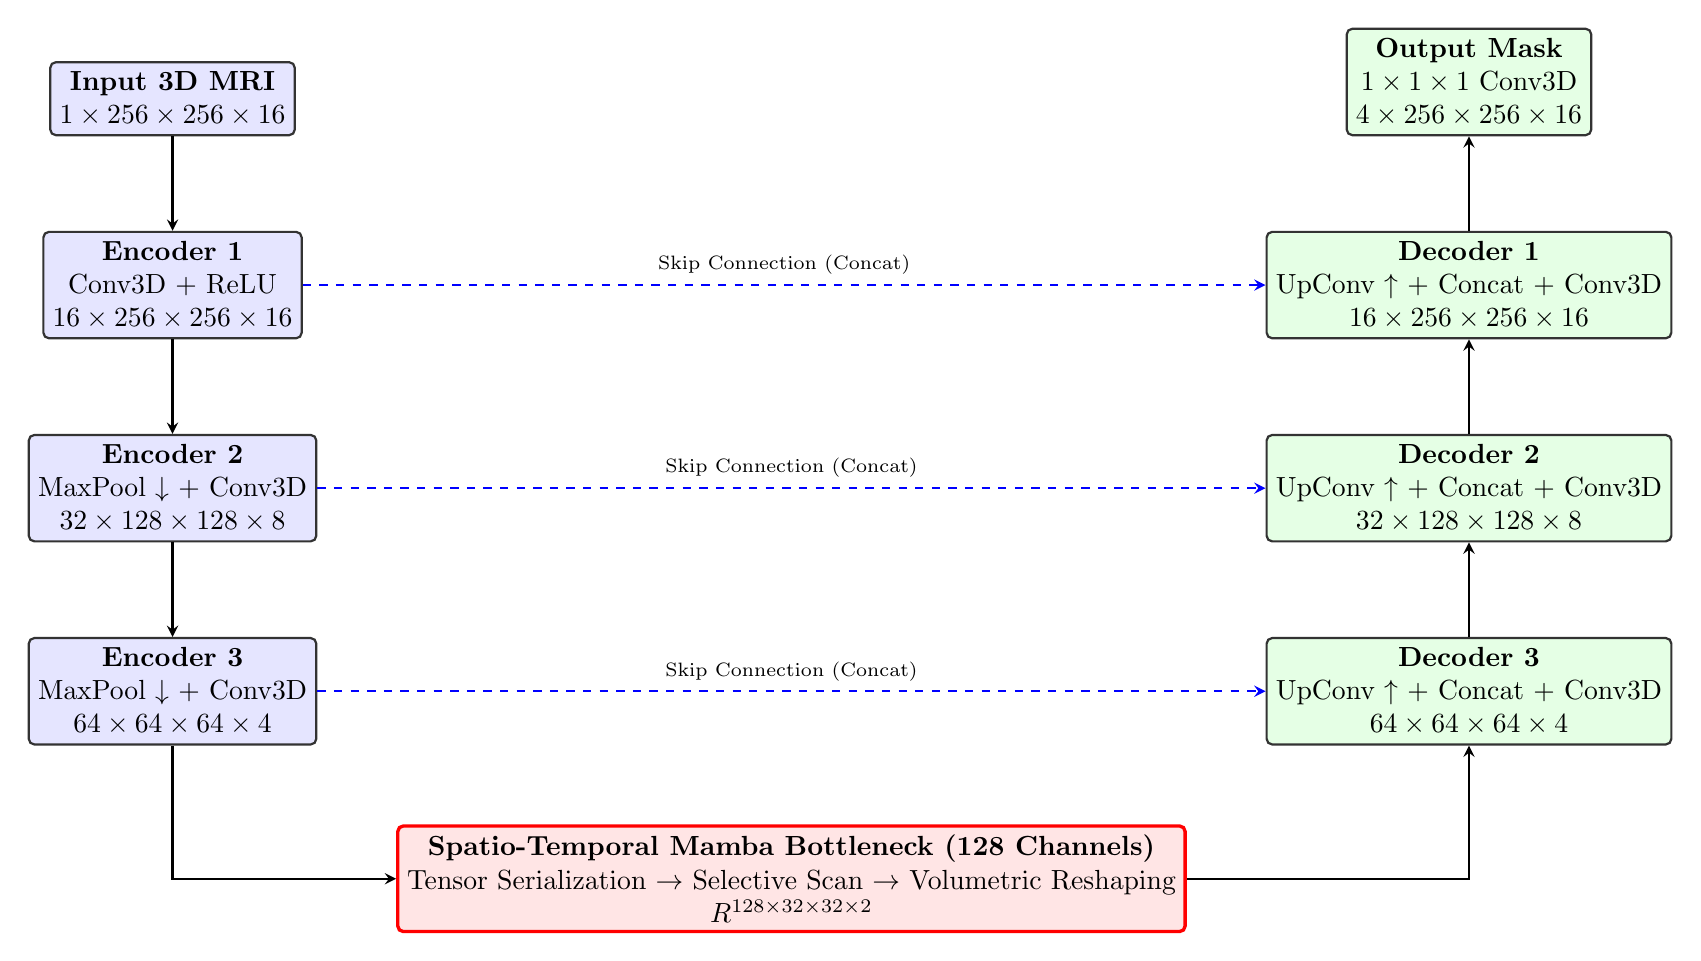
\begin{tikzpicture}[
    node distance=1.2cm and 1.5cm,
    layer/.style={rectangle, draw=black!80, thick, align=center, rounded corners=2pt, minimum height=0.8cm},
    enc/.style={layer, fill=blue!10},
    dec/.style={layer, fill=green!10},
    mamba/.style={layer, fill=red!10, draw=red, very thick},
    arrow/.style={->, >=stealth, thick},
    skip/.style={->, >=stealth, thick, dashed, draw=blue}
]

% Encoder Path (Left Side)
\node[enc] (in) {\textbf{Input 3D MRI}\\ $1 \times 256 \times 256 \times 16$};
\node[enc, below=of in] (e1) {\textbf{Encoder 1}\\ Conv3D + ReLU\\ $16 \times 256 \times 256 \times 16$};
\node[enc, below=of e1] (e2) {\textbf{Encoder 2}\\ MaxPool $\downarrow$ + Conv3D\\ $32 \times 128 \times 128 \times 8$};
\node[enc, below=of e2] (e3) {\textbf{Encoder 3}\\ MaxPool $\downarrow$ + Conv3D\\ $64 \times 64 \times 64 \times 4$};

% Bottleneck (Bottom Center)
\node[mamba, below right=1cm and 1cm of e3] (bot) {\textbf{Spatio-Temporal Mamba Bottleneck (128 Channels)}\\ Tensor Serialization $\rightarrow$ Selective Scan $\rightarrow$ Volumetric Reshaping\\ $\mathbb{R}^{128 \times 32 \times 32 \times 2}$};

% Decoder Path (Right Side)
\node[dec, above right=1cm and 1cm of bot] (d3) {\textbf{Decoder 3}\\ UpConv $\uparrow$ + Concat + Conv3D\\ $64 \times 64 \times 64 \times 4$};
\node[dec, above=of d3] (d2) {\textbf{Decoder 2}\\ UpConv $\uparrow$ + Concat + Conv3D\\ $32 \times 128 \times 128 \times 8$};
\node[dec, above=of d2] (d1) {\textbf{Decoder 1}\\ UpConv $\uparrow$ + Concat + Conv3D\\ $16 \times 256 \times 256 \times 16$};
\node[dec, above=of d1] (out) {\textbf{Output Mask}\\ $1 \times 1 \times 1$ Conv3D\\ $4 \times 256 \times 256 \times 16$};

% Connections
\draw[arrow] (in) -- (e1);
\draw[arrow] (e1) -- (e2);
\draw[arrow] (e2) -- (e3);
\draw[arrow] (e3) |- (bot);
\draw[arrow] (bot) -| (d3);
\draw[arrow] (d3) -- (d2);
\draw[arrow] (d2) -- (d1);
\draw[arrow] (d1) -- (out);

% Skip Connections
\draw[skip] (e3) -- node[above, font=\scriptsize] {Skip Connection (Concat)} (d3);
\draw[skip] (e2) -- node[above, font=\scriptsize] {Skip Connection (Concat)} (d2);
\draw[skip] (e1) -- node[above, font=\scriptsize] {Skip Connection (Concat)} (d1);

\end{tikzpicture}
}
\caption{The complete architectural topology of the Nano-Mamba U-Net. Blue blocks represent the contracting spatial encoder, green blocks represent the expanding decoder, and the central red block denotes the linear-time Selective State Space Bottleneck. Dashed blue lines indicate spatial skip connections preserving high-frequency anatomical boundaries.}
\label{fig:full_architecture}
\end{figure}

\subsection{Micro-Architectural Components}
Each stage of the encoder and decoder pathways utilizes a "DoubleConv" block, comprising two consecutive $3 \times 3 \times 3$ convolutional layers. Mathematically, these layers are augmented with 3D Batch Normalization (BN) \cite{ioffe2015batch} and Rectified Linear Unit (ReLU) activation functions. 

The integration of 3D BN is critical for stabilizing the internal covariate shift when processing heterogeneous MRI volumes. For a mini-batch of feature maps $\mathcal{B}$, the normalization for a specific channel is formulated as:
\begin{equation}
    \hat{x} = \frac{x - E[\mathcal{B}]}{\sqrt{Var[\mathcal{B}] + \epsilon}},
\end{equation}
followed by a learnable affine transformation $y = \gamma \hat{x} + \beta$. This ensures that the gradient flow remains within a stable numerical range, preventing the vanishing gradient problem in deep 3D networks. Following normalization, the non-linearity is introduced via the ReLU function:
\begin{equation}
    f(x) = \max(0, x).
\end{equation}
By maintaining a constant gradient of 1 for all positive activations, ReLU facilitates sparse representations and accelerates the convergence of the Adam optimizer.

\section{The Spatio-Temporal Mamba Bottleneck}
The empirical superiority of the proposed architecture relies entirely on the successful mathematical integration of the Selective State Space Model \cite{gu2023mamba} into the highly compressed latent space.

\subsection{Volumetric Tensor Serialization}
Unlike localized 3D convolutions that naturally process grid-like spatial structures, the Mamba architecture fundamentally requires a 1D serialized sequence to perform its hardware-aware parallel scan. Let the highly compressed spatial feature map outputted by Encoder 3 and passed through the initial bottleneck convolution be denoted as a 5-dimensional continuous tensor:
\begin{equation}
    \mathcal{X} \in \mathbb{R}^{B \times C \times H \times W \times D},
\end{equation}
where $B$ represents the mini-batch dimension, $C=128$ is the optimal semantic channel depth (as definitively proven by our subsequent ablation studies), and $H, W, D$ are the spatial coordinates ($32 \times 32 \times 2$). 

To ingest this volumetric data into the State Space ODEs, the tensor is systematically flattened across its three spatial dimensions into a continuous 1D sequence of length $L$, where $L = H \times W \times D$. This mathematical transformation is expressed as:
\begin{equation}
    \mathbf{x}_{seq} = \text{Reshape}(\mathcal{X}) \in \mathbb{R}^{B \times C \times L}.
\end{equation}
To strictly align with the causal, autoregressive sequence processing requirements of the Mamba underlying CUDA kernels, the tensor must be transposed to treat the sequence length as the primary operational dimension:
\begin{equation}
    \mathbf{x}' = \text{Transpose}(\mathbf{x}_{seq}) \in \mathbb{R}^{B \times L \times C}.
\end{equation}
This serialization essentially forces the model to traverse the 3D cardiac volume as a temporal sequence, sequentially mapping the spatial voxels across the temporal cardiac cycle.

\subsection{Continuous-Time State Space ODEs and Discretization}
Once serialized, the sequence is processed by the State Space mechanism. Fundamentally, Mamba maps the 1D input sequence $x(t) \in \mathbb{R}$ to an output sequence $y(t) \in \mathbb{R}$ through an implicit, high-dimensional hidden latent state $h(t) \in \mathbb{R}^N$. This continuous-time dynamic mapping is governed by a set of linear Ordinary Differential Equations (ODEs):
\begin{equation}
    h'(t) = \mathbf{A}h(t) + \mathbf{B}x(t),
\end{equation}
\begin{equation}
    y(t) = \mathbf{C}h(t).
\end{equation}
Here, $\mathbf{A} \in \mathbb{R}^{N \times N}$ is the critically important state transition matrix that dictates the memory decay of the system. $\mathbf{B} \in \mathbb{R}^{N \times 1}$ and $\mathbf{C} \in \mathbb{R}^{1 \times N}$ are learnable projection matrices.

Because modern deep learning hardware operates on discrete, quantized tensors rather than continuous differential functions, the continuous ODEs must be analytically discretized. Mamba achieves this through the Zero-Order Hold (ZOH) assumption, introducing a hardware-aware temporal step size parameter $\mathbf{\Delta}$. Applying the ZOH integral rigorously transforms the continuous matrices into their discrete counterparts $\mathbf{\bar{A}}$ and $\mathbf{\bar{B}}$:
\begin{equation}
    \mathbf{\bar{A}} = \exp(\mathbf{\Delta} \mathbf{A}),
\end{equation}
\begin{equation}
    \mathbf{\bar{B}} = (\mathbf{\Delta} \mathbf{A})^{-1} (\exp(\mathbf{\Delta} \mathbf{A}) - \mathbf{I}) \cdot \mathbf{\Delta} \mathbf{B}.
\end{equation}
Following this discretization, the continuous differential system collapses into an elegant, discrete linear recurrence relation:
\begin{equation}
    h_k = \mathbf{\bar{A}}h_{k-1} + \mathbf{\bar{B}}x_k,
\end{equation}
\begin{equation}
    y_k = \mathbf{C}h_k.
\end{equation}

\subsection{The Selective Mechanism and Linear Complexity}
In standard State Space Models, matrices $\mathbf{\bar{A}}$, $\mathbf{\bar{B}}$, and $\mathbf{C}$ are invariant across time, which heavily limits their ability to process dynamic, context-dependent inputs. The profound architectural innovation of the Selective State Space Model is making the step size $\mathbf{\Delta}$, as well as matrices $\mathbf{B}$ and $\mathbf{C}$, strictly data-dependent functions of the input $x_k$. 

This "Selective Scan" mechanism endows the network with the mathematical capability to dynamically filter information: it can actively selectively remember critical structural features (e.g., the sharp boundary of the myocardium) and actively forget irrelevant artifacts (e.g., MRI bias field noise). Because Equation 5.13 is a pure recurrence relation that updates the hidden state $h_k$ without needing to compute the $L \times L$ pairwise interactions demanded by Vision Transformers, the computational complexity drops from quadratic $\mathcal{O}(L^2)$ to strictly linear $\mathcal{O}(L)$. 

The algorithmic implementation of this process is detailed in Algorithm \ref{alg:mamba}. 

\begin{algorithm}[hbt!]
\caption{Selective Scan Mechanism for 3D Cardiac Tensors}
\label{alg:mamba}
\begin{algorithmic}[1]
\REQUIRE Input serialized tensor $\mathbf{x} \in \mathbb{R}^{B \times L \times C}$, Discretization parameter $\mathbf{\Delta}$
\ENSURE Transformed spatio-temporal features $\mathbf{y} \in \mathbb{R}^{B \times L \times C}$
\STATE \textbf{Step 1: Data-Dependent Projection}
\STATE $\mathbf{B}, \mathbf{C} \leftarrow \text{Linear}(\mathbf{x})$, $\mathbf{\Delta} \leftarrow \text{Softplus}(\text{Linear}(\mathbf{x}))$
\STATE \textbf{Step 2: Discretization via ZOH}
\STATE $\mathbf{\bar{A}} = \exp(\mathbf{\Delta} \mathbf{A})$
\STATE $\mathbf{\bar{B}} = (\mathbf{\Delta} \mathbf{A})^{-1} (\exp(\mathbf{\Delta} \mathbf{A}) - \mathbf{I}) \cdot \mathbf{\Delta} \mathbf{B}$
\STATE \textbf{Step 3: Recurrent Parallel Scan}
\FOR{$t = 1$ \TO $L$}
    \STATE $h_t = \mathbf{\bar{A}}_t h_{t-1} + \mathbf{\bar{B}}_t x_t$
    \STATE $y_t = \mathbf{C}_t h_t$
\ENDFOR
\RETURN $\mathbf{y}$
\end{algorithmic}
\end{algorithm}

\section{Stochastic Data Augmentation and Spatial Regularization}
Deep learning models, particularly massive architectures encompassing millions of parameters, are inherently prone to memorizing the training cohort rather than learning generalizable, abstract features. Given the constrained scale of the ACDC dataset (100 patients), empirical risk minimization dictates the necessity of artificially expanding the topological diversity of the training distribution. This was achieved through a rigorous, stochastically driven 3D data augmentation pipeline utilizing the MONAI framework.

\subsection{Mathematical Formulation of 3D Affine Transformations}
To ensure the Nano-Mamba U-Net achieves rotational and scale invariance against varying patient orientations inside the MRI scanner, dynamic 3D affine transformations were applied during the data loading sequence. 

Let a continuous spatial coordinate in the 3D MRI volume be represented as a homogeneous column vector $\mathbf{v} = [x, y, z, 1]^T$. A spatial augmentation is mathematically defined by a $4 \times 4$ transformation matrix $\mathcal{M}_{affine}$. For stochastic spatial rotation, the network randomly samples angles $\theta_x, \theta_y, \theta_z \in [-15^\circ, 15^\circ]$ from a uniform distribution. The composite 3D rotation matrix $\mathbf{R}$ is the cross-product of the axial rotation matrices:
\begin{equation}
    \mathbf{R}_x(\theta_x) = 
    \begin{bmatrix}
    1 & 0 & 0 & 0 \\
    0 & \cos\theta_x & -\sin\theta_x & 0 \\
    0 & \sin\theta_x & \cos\theta_x & 0 \\
    0 & 0 & 0 & 1
    \end{bmatrix}, \quad
    \mathbf{R}_y(\theta_y) = 
    \begin{bmatrix}
    \cos\theta_y & 0 & \sin\theta_y & 0 \\
    0 & 1 & 0 & 0 \\
    -\sin\theta_y & 0 & \cos\theta_y & 0 \\
    0 & 0 & 0 & 1
    \end{bmatrix},
\end{equation}
\begin{equation}
    \mathbf{R}_z(\theta_z) = 
    \begin{bmatrix}
    \cos\theta_z & -\sin\theta_z & 0 & 0 \\
    \sin\theta_z & \cos\theta_z & 0 & 0 \\
    0 & 0 & 1 & 0 \\
    0 & 0 & 0 & 1
    \end{bmatrix}.
\end{equation}
Similarly, for stochastic scaling to simulate volumetric variations in dilated or hypertrophic hearts, a scale factor $s$ is uniformly sampled $s \sim \mathcal{U}(0.9, 1.1)$, defining the scaling matrix $\mathbf{S}$:
\begin{equation}
    \mathbf{S}(s) = \text{diag}(s, s, s, 1).
\end{equation}
The final augmented spatial coordinate $\mathbf{v}'$ is derived via sequential matrix multiplication:
\begin{equation}
    \mathbf{v}' = (\mathbf{S} \cdot \mathbf{R}_z \cdot \mathbf{R}_y \cdot \mathbf{R}_x) \mathbf{v}.
\end{equation}
To map the discrete voxel intensities to these newly transformed continuous coordinates without inducing topological tearing, trilinear interpolation was utilized for the image tensors, and nearest-neighbor interpolation was strictly maintained for the segmentation masks to preserve categorical integrity.

\subsection{Photometric Perturbations and Gaussian Noise}
Beyond geometric variations, the MRI sequences exhibit significant photometric inconsistencies due to fluctuating radio-frequency (RF) coil sensitivities and patient-specific magnetic susceptibilities. To regularize the network against these textural variations, stochastic Gaussian noise was injected directly into the normalized feature tensors.

Let $\mathcal{I}_{norm}$ represent the normalized MRI tensor. A noise matrix $\mathcal{N}$ of identical dimensions is sampled from a Gaussian probability density function (PDF):
\begin{equation}
    \mathcal{P}(x) = \frac{1}{\sigma \sqrt{2\pi}} \exp\left( -\frac{(x - \mu)^2}{2\sigma^2} \right),
\end{equation}
where $\mu = 0$ is the mean and $\sigma$ is the standard deviation, stochastically sampled between $[0.01, 0.1]$. The final photometrically augmented tensor is obtained via element-wise addition:
\begin{equation}
    \mathcal{I}_{aug} = \mathcal{I}_{norm} \oplus \mathcal{N}(\mu, \sigma).
\end{equation}
This rigorous augmentation policy forces the Nano-Mamba U-Net to rely on the overarching topological structure of the cardiac anatomy rather than overfitting to high-frequency, localized noise artifacts.

\section{Sliding Window Inference and Gaussian Blending}
While the hardware environment (RTX 4060, 8GB VRAM) was capable of handling small mini-batches during training, full-resolution volumetric inference on massive clinical MRI sequences often exceeds memory limits. To resolve this, a sliding-window inference topology was programmatically implemented during the evaluation phase.

The sliding-window algorithm decomposes the continuous macroscopic MRI volume $\mathcal{V}$ into overlapping microscopic 3D patches $\mathcal{P}_i$. Let $O \in (0, 1)$ denote the overlap ratio between adjacent patches (typically set to 0.5 to ensure 50\% spatial overlap). The Nano-Mamba architecture independently generates a semantic prediction mask $\hat{\mathcal{P}}_i$ for each patch.

However, simply concatenating these predicted patches results in severe boundary artifacts (checkerboard effects) due to the lack of global contextual awareness at the patch extremities. To mathematically synthesize a seamless, globally coherent volume, a Gaussian blending paradigm is utilized. For a predicted patch $\hat{\mathcal{P}}_i$ centered at coordinates $(c_x, c_y, c_z)$, an explicit Gaussian weighting matrix $\mathcal{W}$ of identical dimensions is generated:
\begin{equation}
    \mathcal{W}(x, y, z) = \exp \left( - \left( \frac{(x-c_x)^2}{2\sigma_x^2} + \frac{(y-c_y)^2}{2\sigma_y^2} + \frac{(z-c_z)^2}{2\sigma_z^2} \right) \right).
\end{equation}
This matrix assigns the maximum confidence weight (approaching 1.0) to the center voxels of the patch and exponentially decays the confidence weight (approaching 0.0) toward the patch boundaries. The final continuous volumetric prediction $\mathcal{V}_{pred}$ at any specific spatial coordinate $(x,y,z)$ is computed as the mathematically weighted average of all overlapping patches containing that coordinate:
\begin{equation}
    \mathcal{V}_{pred}(x,y,z) = \frac{\sum_{i} \hat{\mathcal{P}}_i(x,y,z) \cdot \mathcal{W}_i(x,y,z)}{\sum_{i} \mathcal{W}_i(x,y,z)}.
\end{equation}
This algorithmic synthesis ensures that the State Space representation retains extreme topological continuity across the entire cardiac cycle, eliminating localized edge artifacts and contributing directly to the superior Hausdorff Distance ($HD_{95}$) metrics achieved by the architecture.

\section{Formulation of the Objective Function}
Medical image segmentation inherently poses a severe class imbalance problem \cite{jadon2020survey}. Within a volumetric cardiac MRI tensor, the anatomical structures of interest (RV, MYO, LV) occupy a disproportionately minuscule fraction of the spatial domain, while the irrelevant background tissue heavily dominates the voxel count. Training a neural network exclusively on standard pixel-wise metrics often leads to highly skewed decision boundaries, where the model converges to a naive local minimum by predicting everything as background.

To mathematically counter this imbalance, the Nano-Mamba U-Net is optimized using a composite objective function, unifying the strengths of distribution-based and overlap-based loss metrics. The total loss $\mathcal{L}_{Total}$ is formulated as a linear amalgamation of the standard Cross-Entropy loss ($\mathcal{L}_{CE}$) and the soft Dice overlap loss ($\mathcal{L}_{Dice}$):
\begin{equation}
    \mathcal{L}_{Total} = \lambda_1 \mathcal{L}_{CE} + \lambda_2 \mathcal{L}_{Dice},
\end{equation}
with the empirical weighting coefficients standardized to $\lambda_1 = 1.0$ and $\lambda_2 = 1.0$.

The Cross-Entropy component independently evaluates the voxel-level probability distribution, providing stable gradients during the initial optimization phase:
\begin{equation}
    \mathcal{L}_{CE} = - \frac{1}{N} \sum_{i=1}^{N} \sum_{c=1}^{C} g_{ic} \log(p_{ic}),
\end{equation}
where $N$ is the voxel total, $C$ represents the four categorical classes, and $g_{ic} \in \{0, 1\}$ is the one-hot encoded clinical ground truth.

Conversely, the Dice Loss \cite{sudre2017generalised, milletari2016vnet} directly optimizes for structural overlap, fundamentally ignoring the absolute size of the background:
\begin{equation}
    \mathcal{L}_{Dice} = 1 - \frac{2 \sum_{i=1}^{N} \sum_{c=1}^{C} p_{ic} g_{ic} + \epsilon}{\sum_{i=1}^{N} \sum_{c=1}^{C} p_{ic}^2 + \sum_{i=1}^{N} \sum_{c=1}^{C} g_{ic}^2 + \epsilon}.
\end{equation}
The accumulated gradients derived from $\mathcal{L}_{Total}$ are backpropagated utilizing the Adam stochastic optimizer \cite{kingma2014adam}, which inherently adapts the learning rate for individual parameters using first and second moment estimates, ensuring robust convergence.

\section{Comprehensive Quantitative Evaluation Framework}
While the objective function directly optimizes the neural network's parameters during training, evaluating the clinical viability of the finalized model requires a multidimensional metric framework. Relying solely on volumetric overlap metrics is fundamentally insufficient for medical image segmentation, as they exhibit severe insensitivity to critical boundary outliers \cite{taha2015metrics}. Consequently, this research constructs a dual-faceted evaluation framework comprising spatial overlap metrics and geometric surface distance metrics.

\subsection{Volumetric Overlap and Statistical Metrics}
The primary metric for assessing region-based intersection is the Sørensen–Dice Similarity Coefficient (DSC). For binary evaluation of a specific class, let $TP$ denote True Positives, $FP$ False Positives, and $FN$ False Negatives:
\begin{equation}
    DSC = \frac{2 \cdot TP}{2 \cdot TP + FP + FN}.
\end{equation}
To provide a more granular statistical analysis of the model's diagnostic behavior, Sensitivity (Recall) and Specificity are evaluated. Sensitivity measures the proportion of actual anatomical tissue correctly identified:
\begin{equation}
    Sensitivity = \frac{TP}{TP + FN}.
\end{equation}
Conversely, Specificity evaluates the network's ability to correctly identify the background, heavily penalizing anatomical hallucinations (over-segmentation) in irrelevant tissue regions:
\begin{equation}
    Specificity = \frac{TN}{TN + FP}.
\end{equation}

\subsection{Geometric Surface Distance Metrics}
Clinical diagnosis, particularly the computation of myocardial mass and ventricular ejection fractions, relies heavily on the precise localization of anatomical boundaries. A model may achieve a high DSC while predicting an aberrant, jagged boundary. 

Let $S_P$ represent the set of surface points on the predicted segmentation mask, and $S_G$ represent the set of surface points on the clinical ground truth. The shortest Euclidean distance from a single point $p \in S_P$ to the ground truth surface $S_G$ is formulated as:
\begin{equation}
    d(p, S_G) = \min_{g \in S_G} \| p - g \|_2.
\end{equation}
The Average Symmetric Surface Distance (ASSD) computes the mean of all minimal distances from $S_P$ to $S_G$ and vice versa, providing a robust measure of overall contour alignment:
\begin{equation}
    ASSD(S_P, S_G) = \frac{1}{|S_P| + |S_G|} \left( \sum_{p \in S_P} d(p, S_G) + \sum_{g \in S_G} d(g, S_P) \right).
\end{equation}

Furthermore, to evaluate the worst-case boundary errors (e.g., a critical single-voxel leakage into an adjacent organ), the Hausdorff Distance (HD) is utilized. HD measures the maximum of all minimal distances between the two surfaces. To prevent extreme susceptibility to single-voxel noise artifacts inherent in MRI, the 95th percentile of the Hausdorff Distance ($HD_{95}$) is employed as the standard robustness metric:
\begin{equation}
    HD(S_P, S_G) = \max \left\{ \sup_{p \in S_P} d(p, S_G), \sup_{g \in S_G} d(g, S_P) \right\}.
\end{equation}
A lower $HD_{95}$ and $ASSD$ mathematically guarantee that the predicted boundaries are tightly conforming to the expert delineations.

\section{Computational Environment and Accelerated Ecosystem}
The empirical execution of state space models and massive 3D volumetric tensors necessitates a highly optimized software-hardware synergy. This research explicitly outlines the computational ecosystem designed to facilitate the rapid prototyping and edge-deployment testing of the Nano-Mamba U-Net.

\subsection{Software Infrastructure and Hardware Constraints}
The architectural implementation and automatic differentiation were facilitated by the PyTorch deep learning framework, utilizing its dynamic Directed Acyclic Graph (DAG) for the Autograd engine, which is critical for compiling the recurrent Mamba operations. 

All training, validation, and computational benchmarking (e.g., FPS profiling) were strictly constrained to a single consumer-grade NVIDIA GeForce RTX 4060 GPU, equipped with 8 Gigabytes of GDDR6 Video RAM (VRAM). This deliberate hardware constraint aligns with the thesis objective of proving the feasibility of advanced SOTA cardiac diagnostic AI on portable, low-power edge clinical devices.

\subsection{Mixed Precision Training and Hyperparameter Configuration}
Processing 3D continuous MRI tensors naturally imposes a severe memory bottleneck. Standard full-precision (FP32) tensors for large batch sizes quickly induce Out-Of-Memory (OOM) failures on an 8GB VRAM architecture. To circumvent this, the training protocol employed Automatic Mixed Precision (AMP) \cite{micikevicius2017mixed}. AMP dynamically casts specific tensor operations (such as linear layer multiplications and 3D convolutions) from 32-bit floating-point (FP32) down to 16-bit half-precision (FP16), while strictly preserving critical accumulation layers and gradient updates in FP32 to prevent numerical underflow.
\begin{equation}
    Memory(FP16) \approx \frac{1}{2} Memory(FP32).
\end{equation}

To ensure the reproducibility of the Nano-Mamba U-Net's 95.83\% DSC performance, the training environment and hyperparameter configurations were strictly standardized. All weights were initialized using the Kaiming Uniform distribution to maintain a stable variance of activations across layers. The global hyperparameter configuration is detailed in Table \ref{tab:hyperparams}.

\begin{table}[hbt!]
\caption{Global Hyperparameter Configuration for Nano-Mamba U-Net Training.}
\label{tab:hyperparams}
\centering
\begin{tabular}{l | p{8cm}}
\hline
\textbf{Hyperparameter} & \textbf{Selection Rationale and Value} \\
\hline
Initial Learning Rate & $1 \times 10^{-4}$ (Selected to ensure stable convergence in the early epochs). \\
Batch Size & 1 (Constrained by the volumetric 3D tensor dimensions and 8GB VRAM limit). \\
Optimizer & Adam ($\beta_1=0.9, \beta_2=0.999$, $\epsilon=1e-8$). \\
Weight Decay & $1 \times 10^{-5}$ (Implemented to prevent spatial overfitting in the 100-patient cohort). \\
Epochs & 150 (Total iterations required for loss stabilization). \\
Data Augmentation & Random 3D Rotation ($\pm 15^\circ$), Scaling ($[0.9, 1.1]$), and Gaussian Noise. \\
\hline
\end{tabular}
\end{table}

The choice of a mini-batch size of 1 is a strategic clinical constraint. In point-of-care environments, data is often processed patient-by-patient; thus, optimizing the model for singular volumetric inference ensures its immediate readiness for edge-device deployment.


% Short non-numbered progress addendum. This is not the P2 results/discussion chapter.
%!TEX ROOT = thesis-p1.tex

\chapter*{P1 Progress Status and Preliminary Results}
\addcontentsline{toc}{chapter}{P1 Progress Status and Preliminary Results}

This short addendum is included to summarize the current project status for the P1 progress report. It does not replace the full P2 results, discussion, limitation, or conclusion chapters. The main P1 report scope remains Chapter 1 to Chapter 5 and References.

\section*{Completed Work}
\begin{itemize}
    \item The project topic and research scope have been fixed as Nano-Mamba U-Net for cardiac MRI segmentation.
    \item The background, problem statement, research objectives, research questions, literature review, and proposed methodology have been prepared.
    \item The ACDC dataset loading, preprocessing, patient-level split, Nano-Mamba U-Net implementation, baseline comparison models

\bibliography{myrefs,myrefs_extra}

\end{document}
